\documentclass[10pt,a4paper]{jsarticle}
\usepackage{listings}
\usepackage{fancyhdr}
\usepackage{lastpage}
\usepackage[dvipdfm]{graphicx,color}

\lhead{プログラミング実習IIレポート(第6回)}
\rhead{学籍番号:201811433 氏名:西田 直人}
\cfoot{\thepage/\pageref{LastPage}}

\pagestyle{fancy}

\title{プログラミングII実習レポート課題第6回}
\author{西田直人}

\begin{document}
%\markright{プログラミング実習1Aレポート(第1回) 学籍番号:201811433 氏名:西田直人}
%\maketitle
\begin{center}
{\LARGE プログラミング実習IIレポート課題第6回} \\
\large
西田直人 \\ 2018年1月7日
\end{center}
\normalsize
\section{課題6-1}

\subsection{source}
\begin{lstlisting}[basicstyle=\ttfamily\footnotesize,frame=single,breaklines=true]
  //the definition of struct ColoredCircle

  typedef struct ColoredCircle {
    /* 自分で定義する。必要なのは点の座標 xi, yi, 半径 radius および色情報 r, g, b */
  int xi, yi;
  int radius;
  unsigned char r, g, b;

  } ColoredCircle;

  //display function

  void display(void)
{
    int i;
 
    glClearColor(1.0, 1.0, 1.0, 1.0);   /* ウィンドウを消去するときの色を設定 */
    /* ウィンドウを消去 … glClearColor で指定した色で塗りつぶし */
    glClear(GL_COLOR_BUFFER_BIT);
 
    /* for 文で円の個数だけ drawCircle 関数を呼び出して円を描画。自分で実装 */
    for(i=0; i<g_NumCircles; i++){
      drawCircle(g_ColoredCircles[i].xi, g_ColoredCircles[i].yi, g_ColoredCircles[i].radius, g_ColoredCircles[i].r, g_ColoredCircles[i].g, g_ColoredCircles[i].b);
    }
 
    glutSwapBuffers();  /* ここまで指定した描画命令をウィンドウに反映 */
}

//ColoredCircle.c

#include <stdio.h>
#include <math.h>
#include "ColoredCircle.h"

extern void drawCircle(int xi, int yi, int radius, unsigned char r, unsigned char g, unsigned char b);
extern void display(void);


void SetColoredCircle(ColoredCircle *c, int xi, int yi, int radius, unsigned char r, unsigned char g, unsigned char b){
  c->xi = xi;
  c->yi = yi;
  c->radius = radius;
  c->r = r;
  c->g = g;
  c->b = b;
}


int SaveColoredCircles(const char *filename, int n, ColoredCircle circles[]){
  FILE *fp;
  int i, printok;
  
  if ((fp = fopen(filename, "w")) == NULL) {
    fprintf(stderr, "%sのオープンに失敗しました.\n", filename);
    return 0;
  }

  for(i=0; i < n; i++){
    printok = fprintf(fp, "position:(%d, %d) radius:%d color(%d, %d, %d)\n", circles[i].xi, circles[i].yi, circles[i].radius, (int)circles[i].r, (int)circles[i].g, (int)circles[i].b);
      if ( printok < 0 ) {
        fprintf(stderr, "[%d]ファイルの書込みに失敗しました.\n", i);
        fclose(fp);
        return 0;
      }
  }
  
  fclose(fp);
  return 1;
}

int LoadColoredCircles(const char *filename, int *n, ColoredCircle circles[]){
  FILE *fp;
  int i=0, R, G, B;

  if ((fp = fopen(filename, "r")) == NULL) {
    fprintf(stderr, "%sのオープンに失敗しました.\n", filename);
    return 0;
  }


  while(fscanf(fp, "position:(%d, %d) radius:%d color(%d, %d, %d)\n", &circles[i].xi, &circles[i].yi, &circles[i].radius, &R, &G, &B) != EOF){
    circles[i].r = (unsigned char)R;
    circles[i].g = (unsigned char)G;
    circles[i].b = (unsigned char)B;
    i++;
    (*n)++;
  }


  fclose(fp);
  return 1;

}

//Makefile

coloredcircle: circles.o ColoredCircle.o
	cc -o coloredcircle circles.o ColoredCircle.o -lm -L. -I. -lglut -lGL -lGLU -lXi -lXrandr

.c.o:	# サフィックスルール。拡張子 .c から拡張子 .o のファイルを作るためのルール。
	cc -c $<

circles.o: circles.c ColoredCircle.h
	cc -c circles.c ColoredCircle.h -lm

run: coloredcircle
	./coloredcircle
     
\end{lstlisting}

\subsection{result}

\begin{figure}[h]
  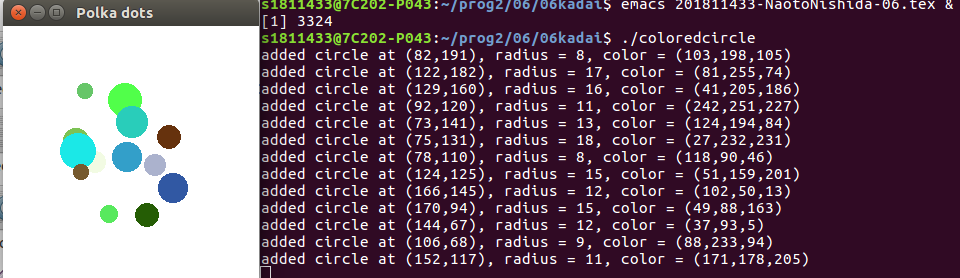
\includegraphics[width=0.8\linewidth]{a.png}
  \caption{最初}
  \label{fig:sutehage}

\end{figure}

\begin{figure}[h]
  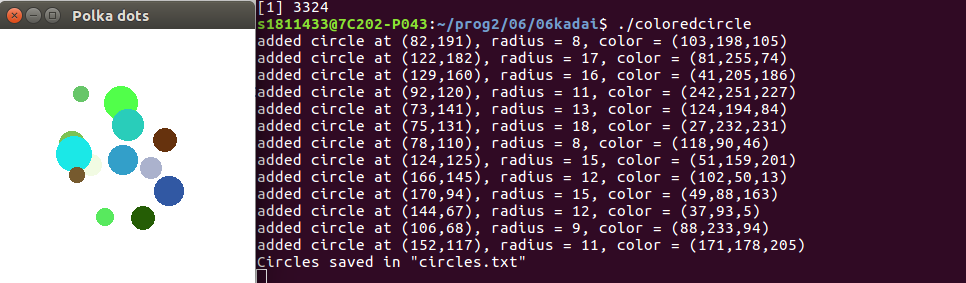
\includegraphics[width=0.8\linewidth]{b.png}
  \caption{数回クリックしたあとにsを押した}
  \label{fig:sutehage}

\end{figure}
\newpage
\begin{figure}[h]
  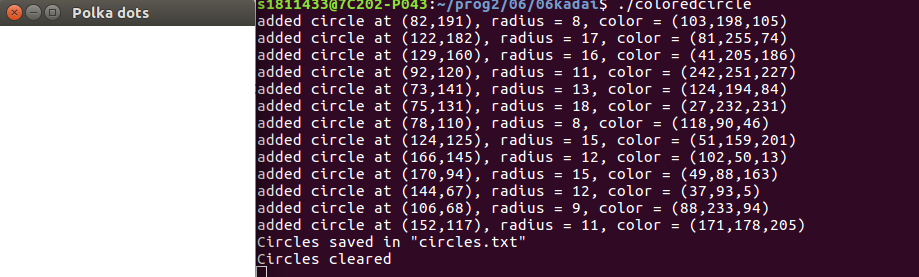
\includegraphics[width=0.8\linewidth]{c.png}
  \caption{スペースキーを押した}
  \label{fig:sutehage}

\end{figure}
\begin{figure}[h]
  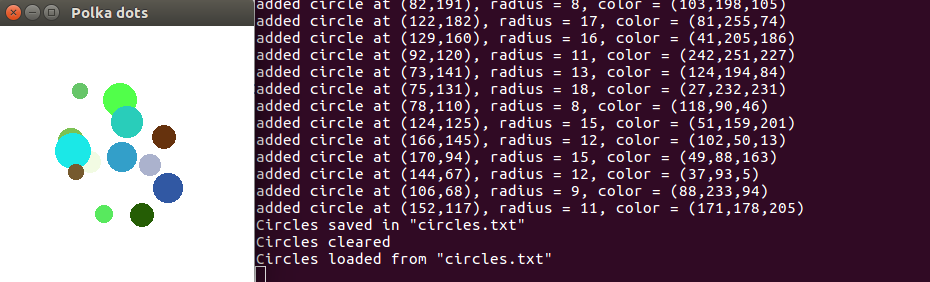
\includegraphics[width=0.8\linewidth]{d.png}
  \caption{lを押した}
  \label{fig:sutehage}

\end{figure}

\newpage

\section{課題6-2}
\subsection{source}
a.
\lstinputlisting[basicstyle=\ttfamily\footnotesize,frame=single,breaklines=true]{csv_dump.c}
b.
\lstinputlisting[basicstyle=\ttfamily\footnotesize,frame=single,breaklines=true\
]{five_opt_quiz.c}
c.
\lstinputlisting[basicstyle=\ttfamily\footnotesize,frame=single,breaklines=true\
]{five_opt_quiz2.c}
header.
\lstinputlisting[basicstyle=\ttfamily\footnotesize,frame=single,breaklines=true\
]{header.h}

\subsection{result}
\begin{lstlisting}[basicstyle=\ttfamily\footnotesize,frame=single,breaklines=true]
  s1811433@LC2RR-P049:~/prog2/06/06kadai$ cc -o csv_dump csv_dump.c
  s1811433@LC2RR-P049:~/prog2/06/06kadai$ ./csv_dump quiz_data_3.csv
  0: Many ubnormal (?) ocurred in this summer.〔この夏は異常現象が頻発した。〕
  phenomena phenomenon ocalts phenix phenixes
  1:
  His company is manufacturing musical (?).〔彼の会社は楽器を製造している。〕
  instruments instructions instructors installations installments
  2:
  For (?) do like this.〔たとえば、こうしてごらん。〕
  example examination exocist exchange exotic
  s1811433@LC2RR-P049:~/prog2/06/06kadai$ ./csv_dump quiz_data_10.csv
  0: Many ubnormal (?) ocurred in this summer.〔この夏は異常現象が頻発した。〕
  phenomena phenomenon ocalts phenix phenixes
  1:
  His company is manufacturing musical (?).〔彼の会社は楽器を製造している。〕
  instruments instructions instructors installations installments
  2:
  For (?) do like this.〔たとえば、こうしてごらん。〕
  example examination exocist exchange exotic
  3:
  The man lived in (?) these days.〔男はその頃ぜいたくな暮らしをしていた。〕
  luxury luck lack lux lacquer
  4:
  The public was in (?) of his policy.〔大衆は彼の政策を支持した。〕
  favor flavor fame fever favorite
  5:
  The experiment failed of (?).〔その実験は必然的に失敗した。〕
  necessity university velocity sensitivity sexuality
  6:
  To tell the (?) Susan is a man.〔本当のことを言うと、スーザンは男だ。〕
  truth lie trust reality hont
  7:
  The human was just an ape in (?).〔ヒトも元々はサルにすぎなかった。〕
  origin virgin orient orientation oracle
  8:
  They will be saved by (?) of love.〔彼らは愛によって救われるでしょう。〕
  means meeting meaning meat method
  9:
  The officer is on (?) now.〔その警官は今勤務中です。〕
  duty dirty destiny debt dusty
  s1811433@LC2RR-P049:~/prog2/06/06kadai$ cc -o five_opt_quiz five_opt_quiz.c
  s1811433@LC2RR-P049:~/prog2/06/06kadai$ ./five_opt_quiz quiz_data_3.csv
  Q1: Many ubnormal (?) ocurred in this summer.〔この夏は異常現象が頻発した。〕
  1:ocalts 2:phenomenon 3:phenomena 4:phenix 5:phenixes
  A1: 3

  Q2:
  His company is manufacturing musical (?).〔彼の会社は楽器を製造している。〕
  1:instruments 2:installments 3:installations 4:instructions 5:instructors
  A2: 1

  Q3:
  For (?) do like this.〔たとえば、こうしてごらん。〕
  1:exocist 2:examination 3:example 4:exchange 5:exotic
  A3: 3

  s1811433@LC2RR-P049:~/prog2/06/06kadai$ ./five_opt_quiz quiz_data_10.csv
  Q1: Many ubnormal (?) ocurred in this summer.〔この夏は異常現象が頻発した。〕
  1:phenix 2:ocalts 3:phenixes 4:phenomenon 5:phenomena
  A1: 5

  Q2:
  His company is manufacturing musical (?).〔彼の会社は楽器を製造している。〕
  1:instructors 2:installations 3:instruments 4:instructions 5:installments
  A2: 3

  Q3:
  For (?) do like this.〔たとえば、こうしてごらん。〕
  1:example 2:examination 3:exocist 4:exotic 5:exchange
  A3: 1

  Q4:
  The man lived in (?) these days.〔男はその頃ぜいたくな暮らしをしていた。〕
  1:lack 2:luxury 3:lux 4:lacquer 5:luck
  A4: 2

  Q5:
  The public was in (?) of his policy.〔大衆は彼の政策を支持した。〕
  1:flavor 2:fame 3:fever 4:favorite 5:favor
  A5: 5

  Q6:
  The experiment failed of (?).〔その実験は必然的に失敗した。〕
  1:necessity 2:velocity 3:sensitivity 4:university 5:sexuality
  A6: 1

  Q7:
  To tell the (?) Susan is a man.〔本当のことを言うと、スーザンは男だ。〕
  1:reality 2:hont 3:truth 4:trust 5:lie
  A7: 3

  Q8:
  The human was just an ape in (?).〔ヒトも元々はサルにすぎなかった。〕
  1:virgin 2:orientation 3:orient 4:origin 5:oracle
  A8: 4

  Q9:
  They will be saved by (?) of love.〔彼らは愛によって救われるでしょう。〕
  1:meeting 2:method 3:meat 4:means 5:meaning
  A9: 4

  Q10:
  The officer is on (?) now.〔その警官は今勤務中です。〕
  1:debt 2:destiny 3:duty 4:dirty 5:dusty
  A10: 3
  s1811433@LC2RR-P049:~/prog2/06/06kadai$ cc -o five_opt_quiz2 five_opt_quiz2.c
  s1811433@LC2RR-P049:~/prog2/06/06kadai$ ./five_opt_quiz2 quiz_data_3.csv
  Q1:
  For (?) do like this.〔たとえば、こうしてごらん。〕
  1:examination 2:exotic 3:example 4:exchange 5:exocist
  A:3
  CORRECT!
  Q2:
  His company is manufacturing musical (?).〔彼の会社は楽器を製造している。〕
  1:instructions 2:instruments 3:installments 4:instructors 5:installations
  A:2
  wrong!
  Q3: Many ubnormal (?) ocurred in this summer.〔この夏は異常現象が頻発した。〕
  1:phenomena 2:ocalts 3:phenomenon 4:phenixes 5:phenix
  A:3
  CORRECT!
  Cleared! (wrong answers: 1)
  s1811433@LC2RR-P049:~/prog2/06/06kadai$ ./five_opt_quiz2 quiz_data_3.csv
  Q1: Many ubnormal (?) ocurred in this summer.〔この夏は異常現象が頻発した。〕
  1:ocalts 2:phenixes 3:phenomena 4:phenomenon 5:phenix
  A:1
  wrong!
  Q2:
  For (?) do like this.〔たとえば、こうしてごらん。〕
  1:exotic 2:examination 3:exchange 4:example 5:exocist
  A:1
  wrong!
  Too many wrong answers, game over...
  s1811433@LC2RR-P049:~/prog2/06/06kadai$ 
\end{lstlisting}


\subsection{分割コンパイル後のソースファイル}
\lstinputlisting[basicstyle=\ttfamily\footnotesize,frame=single,breaklines=true,caption=Makefile2]{Makefile2}
\lstinputlisting[basicstyle=\ttfamily\footnotesize,frame=single,breaklines=true\
  ,caption=csv\_dumpの関数化したやつ]{csv_dumpex.c}
\lstinputlisting[basicstyle=\ttfamily\footnotesize,frame=single,breaklines=true\
  \
  ,caption={five\_opt\_quiz}の関数化したやつ]{five_opt_quizex.c}
\lstinputlisting[basicstyle=\ttfamily\footnotesize,frame=single,breaklines=true\
  \
  ,caption={five\_opt\_quiz2}の関数化したやつ]{five_opt_quiz2ex.c}
\lstinputlisting[basicstyle=\ttfamily\footnotesize,frame=single,breaklines=true\
  \
  \
  ,caption=header.h]{header.h}




\subsection{result}
\begin{lstlisting}[basicstyle=\ttfamily\footnotesize,frame=single,breaklines=true]s1811433@LC2RR-P049:~/prog2/06/06kadai/devidecompile$ make -f Makefile2 run
  ./main quiz_data_3.csv
  which function do you want to use?
  1:csv_dump 2:five_opt_quiz 3:five_opt_quiz2
  1
  0: Many ubnormal (?) ocurred in this summer.〔この夏は異常現象が頻発した。〕
  phenomena phenomenon ocalts phenix phenixes
  1:
  His company is manufacturing musical (?).〔彼の会社は楽器を製造している。〕
  instruments instructions instructors installations installments
  2:
  For (?) do like this.〔たとえば、こうしてごらん。〕
  example examination exocist exchange exotic
  s1811433@LC2RR-P049:~/prog2/06/06kadai/devidecompile$ make -f Makefile2 run
  ./main quiz_data_3.csv
  which function do you want to use?
  1:csv_dump 2:five_opt_quiz 3:five_opt_quiz2
  2
  Q1: Many ubnormal (?) ocurred in this summer.〔この夏は異常現象が頻発した。〕
  1:ocalts 2:phenixes 3:phenomenon 4:phenomena 5:phenix
  A1: 4

  Q2:
  His company is manufacturing musical (?).〔彼の会社は楽器を製造している。〕
  1:instructions 2:instructors 3:instruments 4:installations 5:installments
  A2: 3

  Q3:
  For (?) do like this.〔たとえば、こうしてごらん。〕
  1:exchange 2:examination 3:exotic 4:exocist 5:example
  A3: 5

  s1811433@LC2RR-P049:~/prog2/06/06kadai/devidecompile$ make -f Makefile2 run
  ./main quiz_data_3.csv
  which function do you want to use?
  1:csv_dump 2:five_opt_quiz 3:five_opt_quiz2
  3
  Q1:
  His company is manufacturing musical (?).〔彼の会社は楽器を製造している。〕
  1:instruments 2:installments 3:instructions 4:installations 5:instructors
  4
  A:2
  wrong!
  Q2:
  For (?) do like this.〔たとえば、こうしてごらん。〕
  1:exocist 2:exchange 3:examination 4:example 5:exotic
  4
  A:4
  CORRECT!
  Q3: Many ubnormal (?) ocurred in this summer.〔この夏は異常現象が頻発した。〕
  1:phenixes 2:phenix 3:ocalts 4:phenomenon 5:phenomena
  4
  A:3
  wrong!
  Too many wrong answers, game over...
  s1811433@LC2RR-P049:~/prog2/06/06kadai/devidecompile$
  
     
\end{lstlisting}


\end{document}
